\section{Moving Beyond Flat Index Tags}
\label{sec:background}

%\begin{figure}[t!] 
%\begin{minipage}{1\linewidth}
%\begin{subfigure}[c]{0.96\linewidth}
%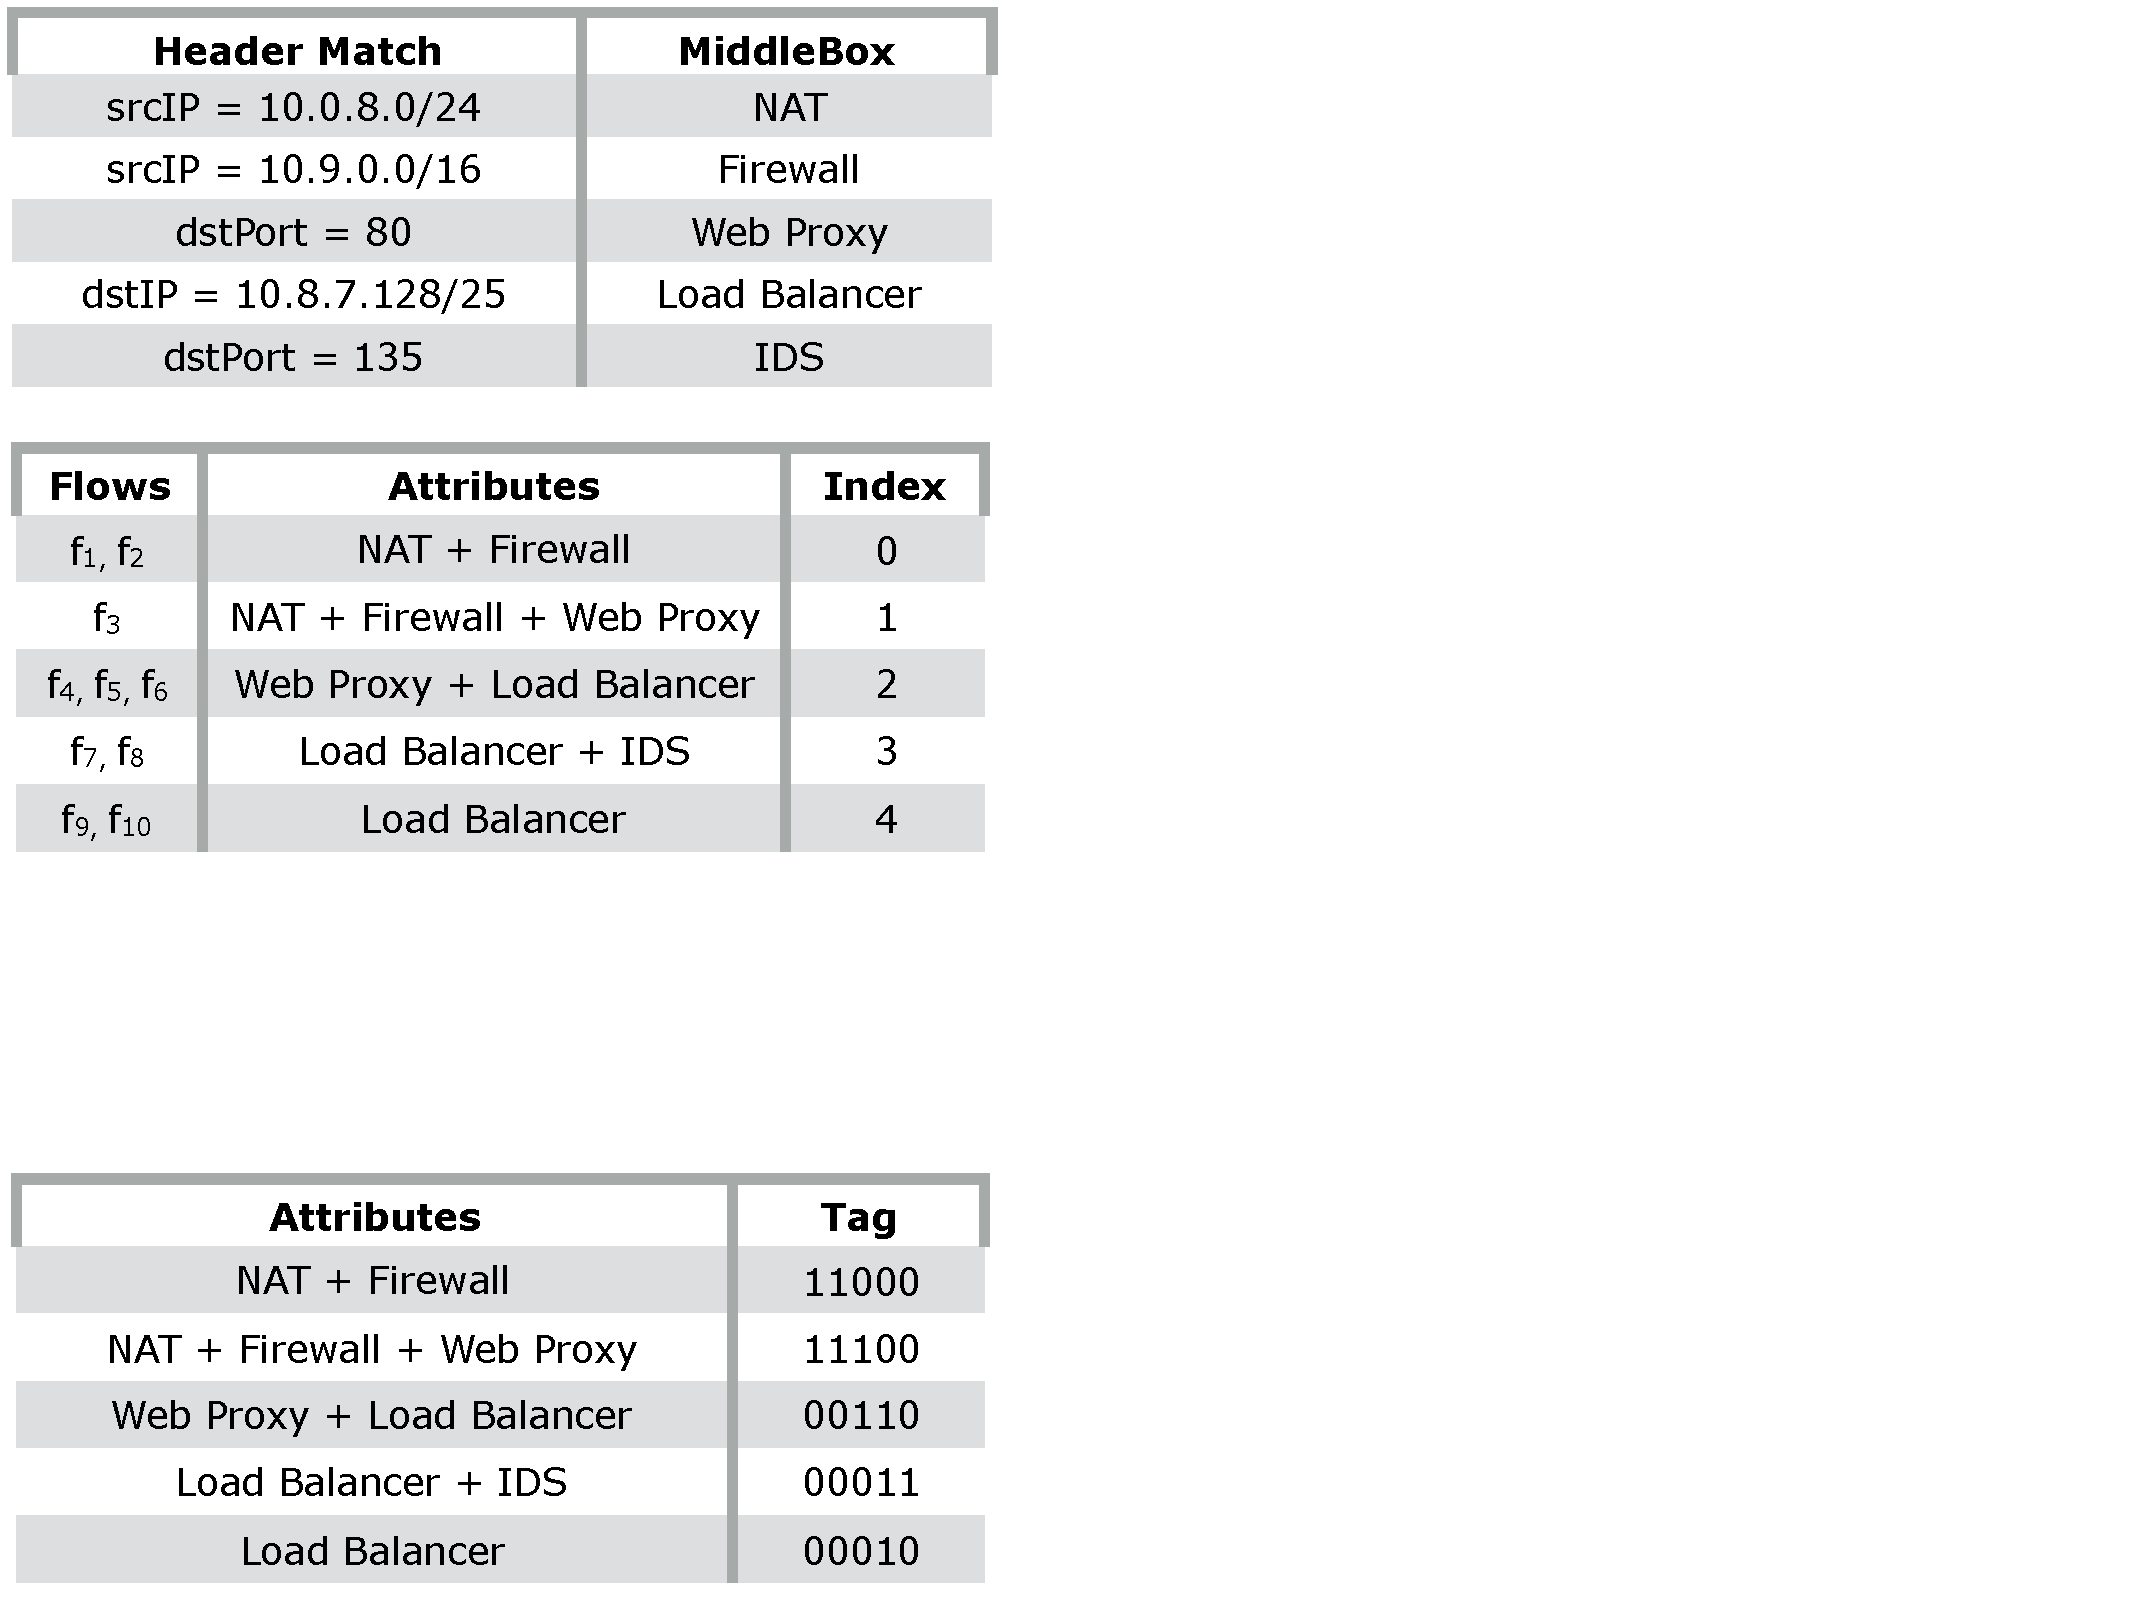
\includegraphics[trim={0 12cm 19cm 0}, clip, width=\linewidth]{figures/mbox_path_example3}
%\end{subfigure} 
%\end{minipage} 
%\caption{In this example, we have a policy that defines traffic which must flow through subsets of five middleboxes. The first table shows which header fields trigger each middlebox, and the second table shows some combinations we may see in network traffic. }
%\label{fig:mbox_policies}
%\end{figure}

Packet labeling schemes need to work within the capabilities of commodity switches.  In this section, we first review packet processing in high-speed switches and how the ``match-action'' capabilities have evolved in recent years.  Next, we discuss flat index tagging and its limitations, and then present several example applications that would benefit from more flexible tagging schemes.

\subsection{Flexible Tags using Flexible Switches}
Commodity switches traditionally use \emph{match-action tables} to determine how to handle packets, based on \textit{forwarding rules} installed at runtime. A table entry consists of a set of match conditions, and an action to take if the matching conditions are met. Actions include dropping a packet, rewriting a header field, or forwarding the packet out a specific port. 
Each matching condition compares a string $S$ to a specific packet header field $H$, using one of three kinds of comparisons:

\begin{itemize}
  \item \textbf{Exact Matching:} $S$ is a binary string, and the match returns true if $S = H$.
  \item \textbf{Longest-Prefix Matching:} $S$ is a ternary string, where the first $x$ characters are binary, and the remaining are the wildcard character $*$. A header field is a match if the $x$ binary characters of $S$ are a prefix of $H$, and there is no other $S'$ in the table which is a longer prefix of $H$. 
  \item \textbf{Wildcard Matching:} $S$ is a ternary string with characters $\{0,1,*\}$ and an associated priority. $S$ matches $H$ if the only characters on which they are unequal are wildcards, and there is no other $S$ in the table which also matches but has a higher priority.
\end{itemize}
  
Until recently, switches imposed significant restrictions on the matching type.  For the vast majority of fields, only exact matching was supported, with the exception of longest-prefix matching for IP addresses. This prevents most fields from being repurposed for anything other than flat tags. However, with recent changes to commodity switches, such as new features supported by OpenFlow 1.3 switches~\cite{of13} and flexible protocol-independent switches~\cite{P4}, we can apply longest-prefix or wildcard matching to existing fields, or even add new fields. Prefix and wildcard matching allows us to treat a header field as a \emph{set} of information, rather than just a single value. 

\subsection{Attribute Equivalence Class Tagging}
%In flat tagging schemes, the tag serves as a single, unstructured index.  A flow of packets is defined by a combination of header fields that each of the packets has in common. Each combination of header fields can imply a set of attributes which are revealed by classification, such as a set of routes the flow may take, middleboxes the flow must traverse, or permissions of the sending/receiving hosts relevant to security policies. 
 Figure ~\ref{fig:mbox_path} shows a simple example of service chaining with four middleboxes, where every flow is mapped to one of four chains by some classification policy. To avoid reclassification at each switch, the figure shows a simple tagging scheme where each of the four paths receives a unique index tag. If the switches have up to date knowledge of which tag maps to which attribute set, reading the tag determines the next-hop. 
 
 In flat tagging schemes, switches must have a rule for each distinct tag they may see. In Figure ~\ref{fig:mbox_path}, the top set of switch rules corresponds to flat tagging. No aggregation of these rules is possible, as flat tagging schemes are based on exact matching rules. 
 
If the switches support more than just exact matching, these rules can be aggregated, as in the bottom set of switch rules. Where flat tagging can require rule space on the order of the number of tags, \emph{flexible tagging} can require as few as a constant action, as seen in in the figure where each next-hop has exactly one corresponding wildcard rule. Of course, this depends entirely upon how the tags are assigned.

\begin{figure}[t!] 
\begin{minipage}{1\linewidth}
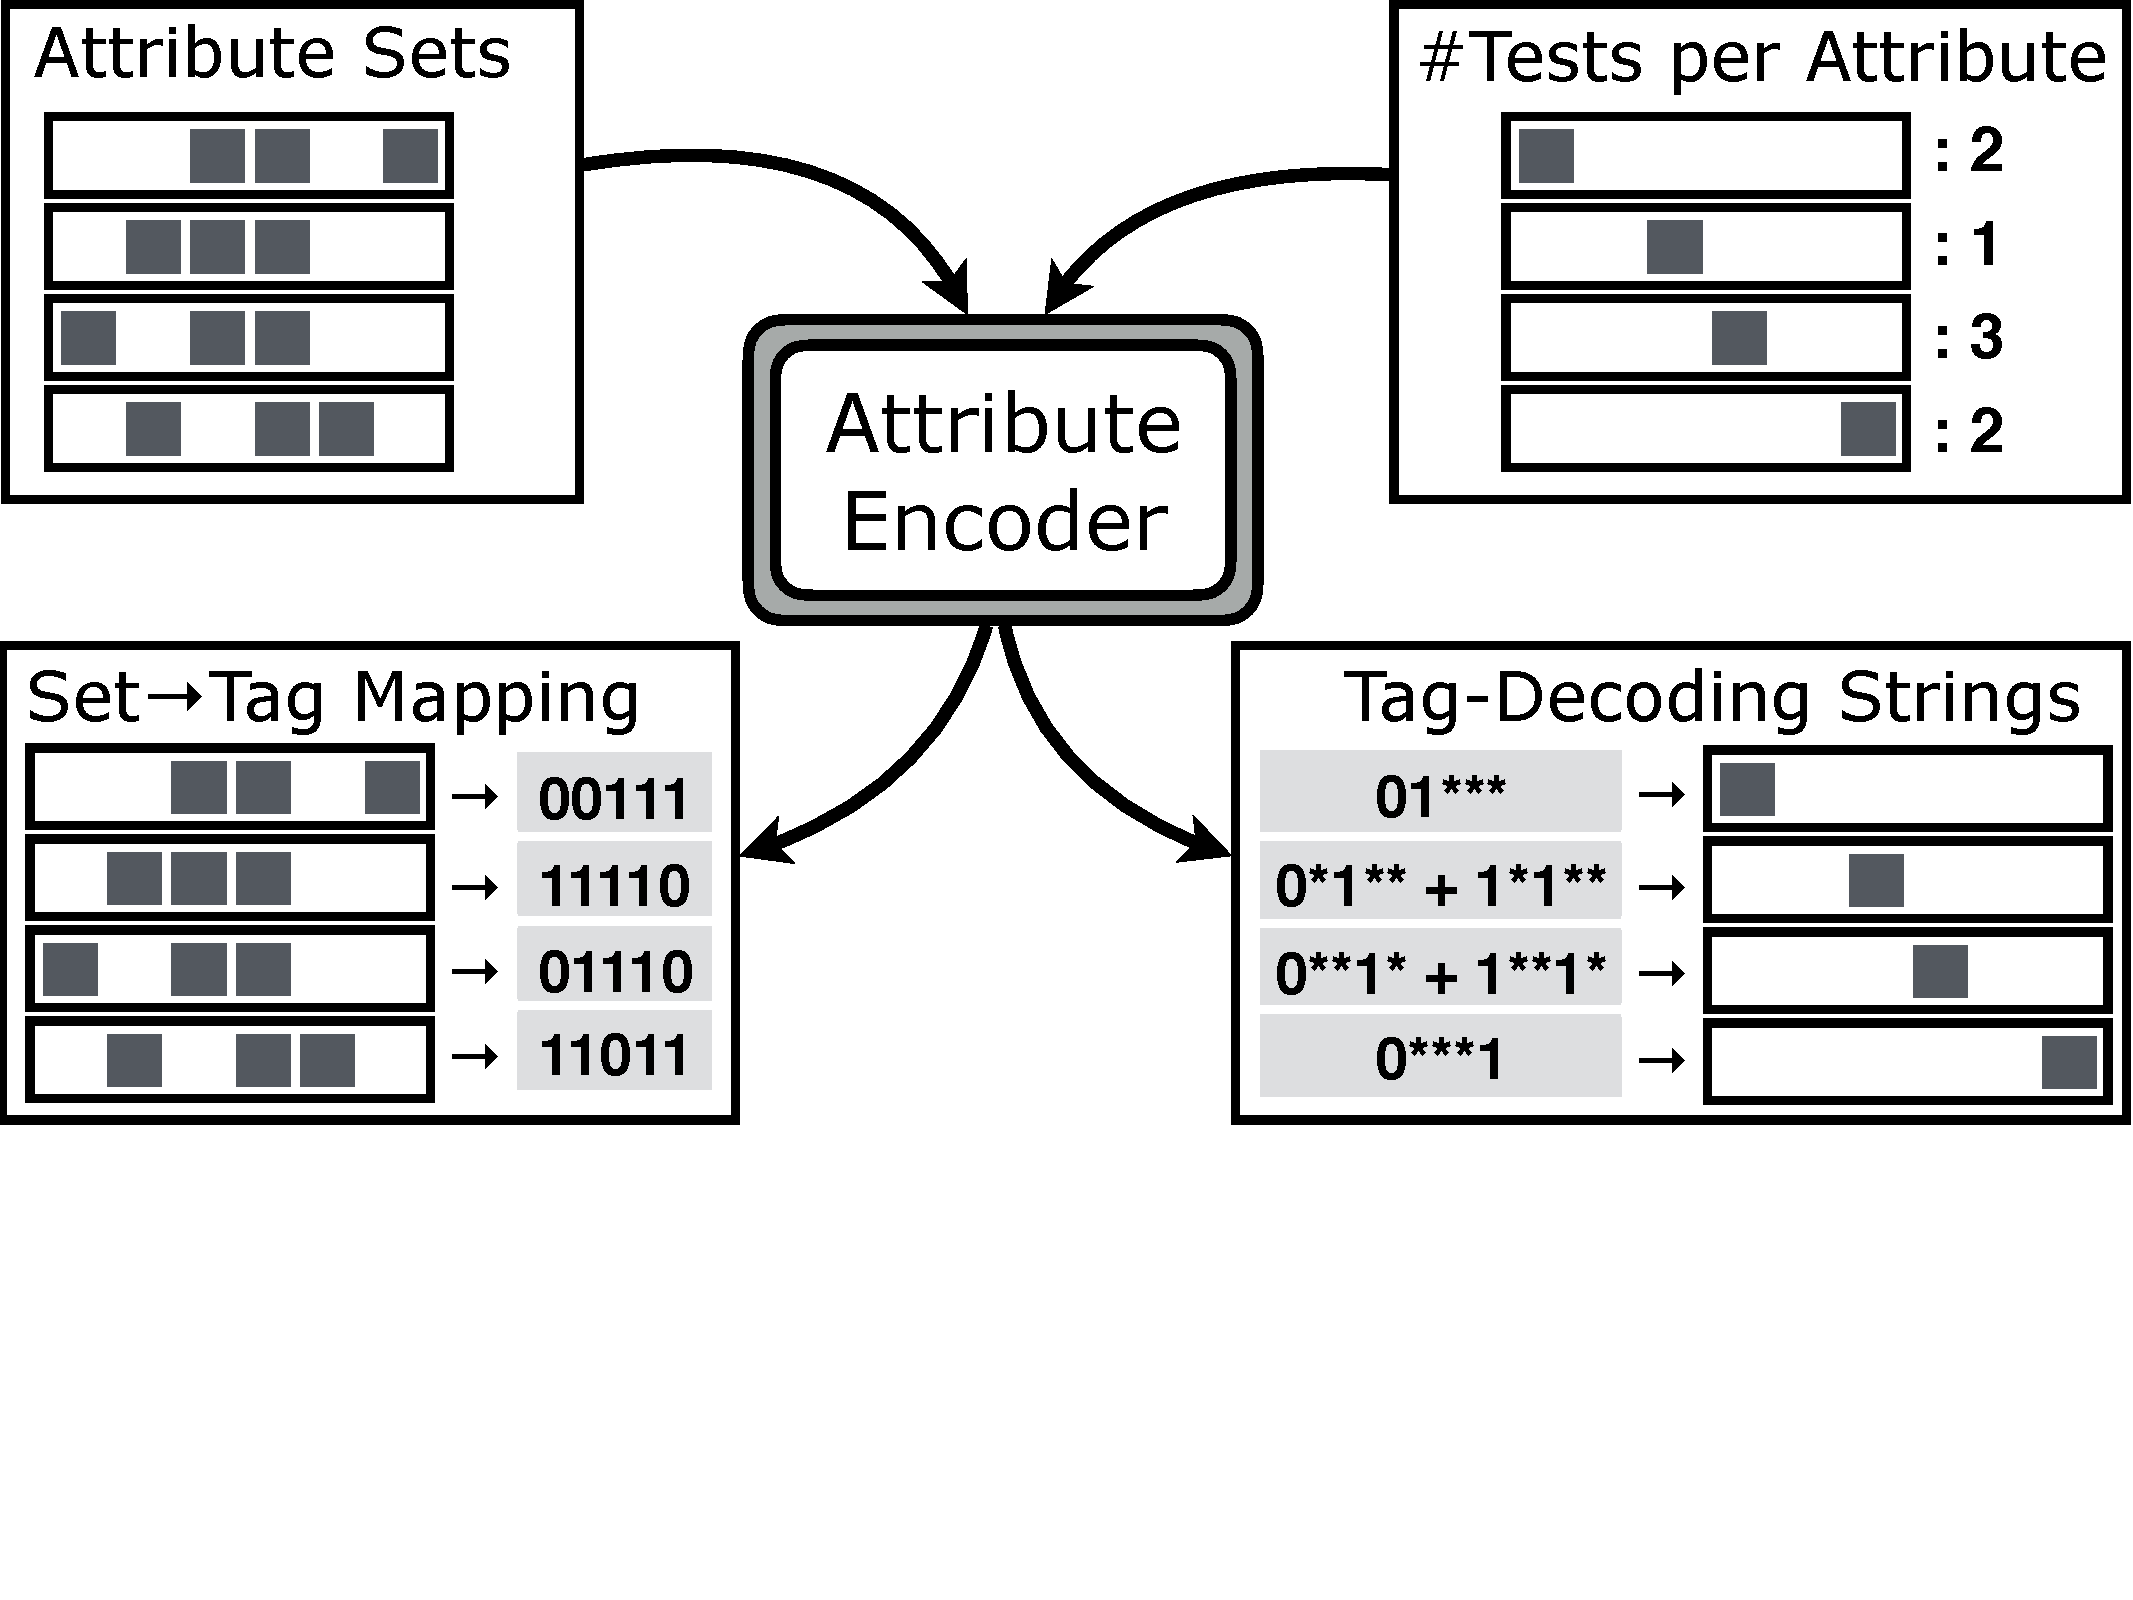
\includegraphics[trim={0 4cm 0 0}, clip, width=\linewidth]{figures/system_flow2}
\end{minipage} 
\caption{An illustration of the information flow for an attribute-encoding tagging scheme. The encoding scheme takes as input a list of attribute sets and the number of queries that will be performed per attribute. The output is a list of tags corresponding to those attribute sets, and wildcard strings used for querying each attribute.}
\label{fig:system_flow}
\end{figure}


\subsection{Strawman Bitmask Tags}

We will now present a strawman tagging scheme which always achieves optimum switch memory usage by using wildcard matches.
If there are $N$ possible attributes to encode in a tag, construct a tag of length $N$: 
the $i^{th}$ bit corresponds to the $i^{th}$ attribute. When the packet is classified
and the tag is attached, the $i^{th}$ bit is set to 1 if the $i^{th}$ attribute
is present for that flow, and 0 if it is not. As a result, if we wish to test for
the presence of attribute $x$, we need only check that $x$'s bit is 1 in the
metadata, rather than exact matching on every tag that contains
$x$.

This approach is a strawman because the tag is of width $N$, and $N$ can be quite large.
Although we criticized flat tagging for using too much switch memory, 
flat tagging only needed tag width logarithmic in the number AECs. We have just traded an extreme in memory
usage for an extreme in tag width. It would be ideal to find some middle ground.
In general, any tagging scheme must simultaneously consider three different metrics:

\begin{enumerate}
\item \textbf{Tag Width:} Tags should not be too wide, to avoid wasting packet-header space.
Tags should be able to either be inserted into small repurposed header fields or contribute little size to custom packet headers. 
\item \textbf{Switch Memory:} The amount of memory required to decode attributes from any tag should be able to easily fit in modern commodity switches rule tables.
\item \textbf{Churn:} Normal network events should not cause the encoding scheme to undergo too many changes.
\end{enumerate}
%It is these metrics by which we will evaluate our solution.
%%%%%%%%%%%%%%%%%%%%%%%%%%%


\section{Motivating Applications}\label{sec:motivation}
\begin{table*}[t]
\begin{center}
    \begin{tabular}{|l|c|c|c|c|}
    \hline
    \multicolumn{1}{|c|}{\bf Application} & 
    \multicolumn{1}{c|}{\bf Attributes} & 
    \multicolumn{1}{c|}{\bf Existing Solution} & 
    \multicolumn{1}{c|}{\bf Tag Field} & 
    \multicolumn{1}{c|}{\bf Tags Conveyed By}\\ \hline
    SDN-enabled IXP & Advertising peers & iSDX~\cite{isdx} & Destination MAC & ARP \\ \hline
    Service chaining & Middleboxes & FlowTags~\cite{flowtags} & IP Fragment Field & First Middlebox \\ \hline
    Policy enforcement & Host permissions & Alpaca~\cite{alpaca} & IP Source Address & DHCP \\ \hline
    \end{tabular}
\end{center}
    \caption{Example applications and systems which have solved them by some form of tagging.} 
    \label{tab:applications}
\end{table*}

There are many applications where encoding and reading AECs is of interest, and in particular we will look at three of them, which are outlined in Table \ref{tab:applications}.
 
\paragraph{Software-Defined Internet Exchange Points}
At an Internet Exchange Point (IXP) multiple autonomous systems (ASes) connect at a single point to exchange traffic and interdomain routing information as peers.  At an IXP with support for SDN policies, the connected ASes may wish to enact fine-grained routing policies, where routing is decided by more than just destination addresses. Say that $AS_1$ wishes to send as much of their HTTP traffic to $AS_2$ as possible. $AS_2$ may not have routes to every HTTP destination, so it is incorrect for them to receive all HTTP traffic. If the routing policies do not account for the routes of each AS, traffic may be forwarded to networks that cannot handle it. 

The SDX project~\cite{sdx} handles this issue with the use of index tags. Each AS shares its list of routes with a central controller, and every unique set of routes is assigned an index tag. The controller then attaches these tags to every packet by announcing them to all peers as destination MAC addresses via ARP replies. The fine-grained routing policies are then modified by the controller to read tags before making a routing decision. 

The index tagging scheme of the original SDX ran into memory scalability challenges as a direct result of index tagging, which were remedied by the followup work iSDX~\cite{isdx}. iSDX used a precursor to our tagging scheme, taking advantage OpenFlow 1.3's support for wildcard matching on destination MAC addresses. 

\paragraph{Service Chaining}
Network operators often desire that network traffic be directed through a series of middleboxes, such as load balancers or firewalls. Such middleboxes can provide security and performance guarantees for the network's users.
 Different flow may be subject to different chains of middleboxes, and it can be a challenge to design the network in such a way that every flow traverses only the needed set of middleboxes. Additionally, middleboxes may modify packet headers, obscuring the original source of the flow and making it unclear which middlebox chain should be followed. 
 
FlowTags~\cite{flowtags} argues that a necessary remedy is the modification of middleboxes to attach relevant policy information to packets as they are processed. To compress policy information into small, repurposed header fields, flowtags makes use of index tagging, where each index maps to a middlebox sequence and the packet's origin host. Each time a middlebox sees a new flow, it communicates with a central controller to establish a new index tag. 
However, the FlowTags paper does not evaluate the number of forwarding table entries required by network switches to determine which middleboxes a packet should be forwarded to. It is worth exploring the benefits such a system could see from a different tagging scheme. 
 

\paragraph{Host Attributes for Network Policies}
In some situations, network policies require knowledge of properties of sending hosts to be correctly enforced. As an example, users in different departments of a university may be subject to different quality of service or access control policies. If department information is not attached to packets directly, it must be inferred from some combination of packet header fields, which can result in unnecessarily complex forwarding tables. 

The Alpaca~\cite{alpaca} paper addresses this by encoding policy information in IP addresses, and assigning these addresses to network hosts via DHCP. Although not explicitly a tag, these IP addresses can be thought of as a tag appended to the network's IP prefix. Alpaca takes advantage of prefix and wildcard matching in construction of their "tags" to circumvent the memory scalability challenges of index tagging, however their approach has the added constraint that each host must receive a different tag, because each IP must be unique. The work does not consider what is possible using prefix and wildcard matching if the tags were unique per FEC, rather than per host.


%\paragraph{Multicast and Anycast}
%In a classic IP anycast scenario, a single service is replicated across multiple servers to attempt to lighten the maximum load that any single server receives. Since each server hosts the same server, they can all equivalently handle packets destined for that service. Each server is assigned the same IP address, and the network forwards any traffic destined for the shared IP address to the nearest replica of the service. However, if each server has a set of services it replicates, but sets differ across servers, no two servers can be treated equally and receive identical IP addresses. If lists of servers could be attached to packet headers, the network could read this list and choose a server to handle the packet. 
%The scenario of Multicast is similar, where a list of subscribers can be attached to the packet header of a multicast packet. The network would then read this list and replicate the packet towards each subscriber. 